\noindent
\begin{tabular}{cc}
\begin{minipage}[b]{0.60\textwidth}
\begin{exerciseS}
Dato il condotto a sezione circolare rappresentato in figura, 
determinare la portata in massa d'olio, $\overline{\rho} = 850\ kg/m^3$,
attraverso il condotto stesso sapendo che il diametro del condotto 
\`{e} $D=0.5\ m$, che la differenza di altezza fra i peli liberi 
\`{e} $H=40\ cm$, che il diametro del tubo a U \`{e} di $2$ mm. 
Si trascuri qualunque effetto dissipativo, si assuma
uniforme la velocit\`{a} in una sezione sufficientemente lontana a monte
e si consideri che nel tubo a U sia presente aria in condizioni normali.

($\overline{Q}= 467.2\ kg/s$)
\end{exerciseS}
\end{minipage}
&
\begin{minipage}{0.35\textwidth}
   \begin{center}
   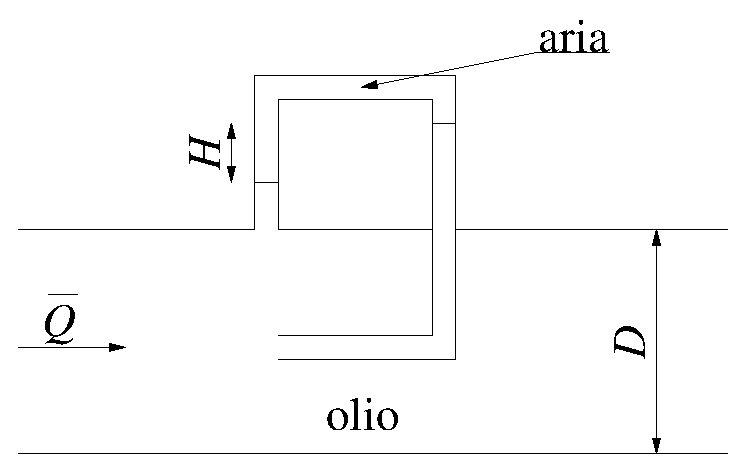
\includegraphics[width=0.90\textwidth]{./fig/condottocircolare.eps}
   \end{center}
\end{minipage}
\end{tabular}

\sol

\partone
 Teorema di Bernoulli nell'ipotesi di stazionarietà, fluido incomprimibile, non viscoso, irrotazionale.
Equazione della vorticità nel caso non viscoso.
Legge di Stevino.

\parttwo
Il problema viene risolto con l'applicazione del teorema di Bernoulli (ipotesi...; eq. della vorticità:...) e della legge di Stevino all'interno del tubo "a U".

Alcune "ipotesi gemoetriche" e sul campo di moto...(continuità soddisfatta)

Sulla linea di corrente che incontra l'imbocco del tubicino, il fluido subisce un rallentamento dalla velocità di ingresso fino ad arrestarsi.

Vengono definiti i punti $0$ coincidente con la presa del tubo all'interno del canale; $1$ il punto infinitamente a monte sulla linea di corrente che arriva al punto $0$; $2$ il pelo libero di sinistra all'interno del tubo "a U", $3$ il peo libero di destra. Si definiscono anche $h_2$ e $h_3$ come quote dei peli liberi sulla linea di corrente congiungente $0$ e $1$ (oss. $H = h_3 - h_2$).
Il sistema risolvente è:
\begin{equation}
\begin{cases}
  P_1 + \frac{1}{2} \rho U^2 = P_0 \\
  P_3 - P_0 = -\rho g h_3 \\
  P_2 - P_1 = -\rho g h_2 \\
  P_3 - P_2 = -\rho_a g H \\
  \bar{Q} = \rho \frac{\pi}{4}D^4 U
\end{cases}
\end{equation}

Risolvendo per U:
\begin{equation}
  \frac{1}{2} \rho U^2 = P_0 - P_1 = ... = (\rho - \rho_a) g H \quad \Rightarrow \quad 
  U = \sqrt{2\displaystyle\left(1-\frac{\rho_a}{\rho}\right) g H}
\end{equation}

Inserendo i valori numerici: $U = 2.799 m/s$, $\bar{Q} = 467.15 kg/s$.


